\documentclass[aps,prd,onecolumn,fleqn,superscriptaddress,groupedaddress,nofootinbib,preprintnumbers,nobalancelastpage]{revtex4}
\pdfoutput=1
\usepackage{amsmath,amssymb,pstricks,graphicx}

\begin{document}
\preprint{SLAC-PUB-?????, MCNET-18-??}
\title{Precision comparisons of predictions for Z/H + jet
and di-jet production at the LHC as a function of jet size}

%\author{Johannes Bellm}
%\affiliation{Lund University}
%\author{Xuan Chen}
%\affiliation{University of Zurich}
%\author{James Currie}
%\affiliation{University of Zurich}
%\author{Aude Gehrmann-De Ridder}
%\affiliation{ETH Zurich}
%\author{Thomas Gehrmann}
%\affiliation{University of Zurich}
%\author{Nigel Glover}
%\affiliation{IPPP Durham}
%\author{Alexander Huss}
%\affiliation{CERN}
%\author{Joao Pires}
%\affiliation{Instituto Superior Tecnico}
%\author{Stefan H{\"o}che}
%\affiliation{SLAC National Accelerator Laboratory}
%\author{Joey Huston}
%\affiliation{Michigan State University}
%\author{Silvan Kuttimalai}
%\affiliation{SLAC National Accelerator Laboratory}
%\author{Simon Pl{\"a}tzer}
%\affiliation{University of Vienna}
%\author{Emanuele Re}
%\affiliation{LAPTH Annecy-le-Vieux}
  
\begin{abstract}
  We perform a phenomenological study of
  $Z$ plus jet, Higgs plus jet and di-jet production
  at the Large Hadron Collider. We investigate in particular
  the dependence of the leading jet cross section on the
  jet radius as a function of the jet transverse momentum. 
  Theoretical predictions are obtained using perturbative QCD
  calculations at the next-to and next-to-next-to-leading order.
  They are compared to results obtained from matching 
  next-to-leading order calculations to parton showers.
\end{abstract}

\maketitle

\section{JH comments}

\subsection{Preamble for paper}

We expect ME+PS predictions to differ from the underlying ME predictions in regions where (1) there is a large sensitivity to jet shapes (typically small R jets), (2) there is a restriction in phase space such that soft gluon resummation effects are important, (3) the observable contains multiple, disparate  scales, (4) the observable depends on a higher multiplicity final state than can be produced by the matrix element. Such differences should be smaller at NNLO than at NLO. The corollary would be that, except for (4), the other effects result in 
potentially large logs. Large parton shower effects in the absence of such large logs should be viewed with suspicion, as should large differences between parton shower predictions in general. Thus, it is useful to compare ME+PS predictions with their underlying fixed order backbone. 

JB: We further expect the ME+PS and ME predictions differ from full simulations when multiple parton interactions (MPI) (small $p_T$ and/or large R) or hardonisation  (small $p_T$ and/or small R) effects become important. 

\subsection{Introduction for paper}

A contribution to LH17 compared predictions for H+j production at LO, NLO and NNLO to those from Sherpa and Herwig7, for a variety of jet radii. Good agreement was observed between Sherpa and Herwig7, and between the two ME+PS predictions and the fixed order predictions, modulo the incomplete description of the jet shape provided by the fixed order predictions. The best agreement between ME+PS and fixed order was obtained with the NNLO predictions, as expected given its more complete description of the jet shape. In this paper, we follow up with further comprehensive comparisons for H+j, and for two additional processes, Z+j and dijet, concentrating on inclusive observables, such as the lead jet transverse momentum distribution. Contrary to popular opinion, the agreement among the various ME+PS predictions (including Powheg for dijet production) for these observables is good, as is the underlying agreement with the relevant fixed order predictions, especially at NNLO. 

In addition, we examine the scale uncertainties of the three processes, at LO, NLO and NNLO, as a function of jet radius, and comment on the implication of our results on the $\it reasonable$ determination of the scale uncertainties. 

\subsection{Comments from Oct 15}

The question was raised in our last meeting as to what our goals should be for this paper. I said I would come up with something to start. Please add to this list as you see fit. 

I was connected to the LHC EWWG meeting on jets and EW bosons this morning, and mentioned this study. They seemed to be interested to have a presentation for one of the biweekly meetings and/or the 2-day meeting at CERN in December. 

First, refer back to our LH17 contribution. We would like to duplicate the figures shown there for H+jet, with Z+jet and dijet production, as much as possible. 

\begin{itemize}
\item 

Fig. V.14

K-factors for Z,  and for lead jet from Z+jet, and for inclusive jet production, all as a function of pT; compare to K-factors for H, lead jet from H+jet (by eye, or with a separate plot?)

\item
Fig. V.16

reproduce LO, NLO, NNLO curves for R=0.4,0.7,1.0; for Z production we could also scale using the K-factors for Z $p\gt$150 GeV/c; does it make sense to do that for inclusive jet production as well? 

\item
Fig. V.17

reproduce for Z+jet, inclusive jet; new figure: compare the scale uncertainty envelopes for the 3 processes as a function of R at fixed pT; try several values of pT;  absolute uncertainty/normalized to the uncertainty for each process at R=0.7

\item

Fig. V.18/V.19

should we normalize to R=0.7 for Z+jet, incl jet? maybe constructing the RHS of V.19 would tell us

reproduce V.18 and V.19 (of course top half of plot doesn't exist for incl jet); for Higgs, can we try re-weighting V.19 (left) for the finite top mass theory

\item
Comparison plots:

for each process, show cross sections for R=0.3-1.0 as a function of jet pT; linear plot showing NLO, Sherpa, Herwig, Powheg normalized to NNLO



\end{itemize}

\subsection{Comments regarding new plots from Johannes/Stefan}

\begin{itemize}
 
 \item 

Comparison Plot

It’s interesting that the R-dependence is:

-significantly larger at NNLO than at NLO for H+j
-is much smaller for Z+j than for H+j; quark vs gluon jets? 
-is similar at NNLO and NLO for inclusive jet production; NNLO comparable to H+j; NLO larger than the other two processes

It may be useful to produce jet shape plots for Z+j and inclusive jet similar to Fig. V.15 in the Les Houches writeup. 

Fig. V.14 in the LH writeup only looked at the ratios of NNLO/NLO as a function of R

\item 

Comparison Contributions

No specific comments other than dijet production differs from the other two processes in the relative quality of the lead two jets. 

\item

Fig. V14 Higgs 2

Interesting that Sherpa and Herwig7 agree so well with FO NLO  above 100 GeV/c for Higgs pT. Should we also compare for the lead jet pT for H+j? Look for different R values? 

\item 

Fig. V14 Z 2

Similar comments as for previous figure. Considerable slope for NLO/LO as a function of pT of lead jet due to increasing dominance of dijet configurations. Look at this for other R values? 

\item

Fig. V14 J2

No specific comments other than again Sherpa, Herwig7 (and now Powheg) agree well with each other and with FO NLO. Look at this for other R-values?

\item

Fig. V16 Higgs

from LH17 writeup; note that for F=0.4 Sherpa and Herwig7 tend to be near the bottom of the scale uncertainty band at LO, NLO and NNLO

\item 

Fig. V16 ZJ

for R=0.4, Sherpa and H7 below error band at NLO and NLO; error band vanishingly small at NNLO

\item 

Fig. V17 Higgs

from LH17 writeup

scale uncertainty grows as R increases as expected; scale uncertainty never goes to 0; slopes steeper at NNLO than at NLO;  Sherpa/Herwig slope similar to NNLO

\item 

Fig. V17 Z

same comments as above, but scale uncertainty vanishes at R=0.3

\item

Fig. V17 InclJet 196.0

same comments as above, except that: (1) scale uncertainty vanishes at R=0.4, (2) now have Powheg which agrees with Sherpa and Herwig, except that Powheg slope is a bit steeper at high R
(is this significant?); note that this is for one scale, muR=HT/2,muF=HT/4. We want to produce FO curves using the other scales that Joao provided, even though we are not varying the scales for the ME+PS predictions. 

\item 

Fig. V18 Higgs

from LH17 writeup

R variation larger for Sherpa/Herwig than for FO, even at NNLO; surprising that FO R=1.0 is smaller (relative to R=0.7) than Sherpa/Herwig?

\item

Fig. V18 Z

again, FO R=1.0 smaller than Sherpa/Herwig

\item

Fig. V18 inclJet

much larger R variations for inclusive jets than for Hj/Zj; is the reason just that there are two jets at the Born level? 

\item

Fig. V.19 from LH17 also exists for Z+j (Johannes made it); we should also make for dijet production

\end{itemize}

We have a somewhat unique sample of the scale uncertainty as a function of R, at LO, NLO and NNLO for three processes. In addition, we have 3 choices of scale function at NNLO for inclusive jet production. This hopefully will contribute to the discussion/understanding of determining a reasonable scale uncertainty for the very precise NNLO calculations that are currently available. Below I pasted the content of an email message that I previously had sent out. 

As an additional figure, similar to V.17:

Separate plots for each of the three processes of  the scale uncertainty envelopes, as a function of jet pT, for the different values of R. Try combining the three processes into one plot; may involve restricting the number of R values used. For inclusive jet, separate plots for central scale choice of pT,pT1
and HTpartons, as a function of R, which all should be available in the information provided by Joao. 

Below starts some text from the original LH17 document that Stefan put in. 

\section{Introduction}
During Les Houches 2015~\cite{Badger:2016bpw}, a detailed 
comparison of fixed order (at NLO and NNLO) and matrix element plus parton shower (MEPS) predictions for differential Higgs
boson (+jet) production was carried out. The goal was multi-fold: using identical
starting configurations, to check the consistency of the MEPS
predictions among themselves, and to demonstrate that that the MEPS
predictions revert to their underlying fixed order predictions in
non-Sudakov kinematic regions. 
These comparisons largely showed good agreement among the ME+PS predictions and 
 that the ME+PS predictions agreed reasonably well with their fixed order counterparts. 

We have continued these studies in Les Houches 2017, but now looking in finer detail at 
the level of agreement. In particular, the perturbative jet shape is not as
well-defined at fixed order as with the NLO matrix element plus parton shower
predictions that are available. This may have a quantitative impact on the cross
section predictions, especially for small jet sizes.   

The study is designed to use Higgs+jet, Z+jet and inclusive jet production,
taking advantage of the NNLO calculations available for all three processes.
% It
%will be interesting to examine whether the good agreement between fixed order
%and ME+PS predictions observed for H+jet in the 2015 study holds for Z+jet and
%inclusive jet. 
The latter two processes are important for global PDF fits, where
only fixed order predictions (along with the relevant non-perturbative
corrections) have been used. 
Due to time constraints, only the Higgs+jet process will be considered in detail
in these proceedings. The other two processes, along with Higgs+jet,  will be
included in a more comprehensive study in a future publication. 

As a  further test of the impact of parton showers versus fixed order, the jet
size was varied over the values 0.3,0.4,0.5,0.6,0.7,1.0, using the antikT jet
algorithm. Indirectly, this tests how well the one (two) extra gluon(s) at
NLO(NNLO) reproduce the perturbative aspects of the jet shapes, as embodied by
the parton shower. This is of particular interest as the Higgs boson + jets measurements that have been performed at the LHC in Run 2 have used a jet size of 0.4, which is 
slightly above the jet size region where small R effects may be important. Taking them into proper account would require resummation, as discussed in ~\cite{}. The MEPS predictions also basically provide this resummation, through the parton showers. The 
MEPS predictions at NLO can properly take these effects into account. However, the highest precision for $H+\ge1$ jet is from the NNLO predictions, and there is no MEPS formalism that works at this order.   As an additional motivation, there has been recent speculation that the quark jet shape is
not well-described at NLO. This study provides samples of both quark and gluon
jets to test this hypothesis.

  Predictions from MEPS programs were carried out
at the parton shower level (for easiest comparison to fixed order)~\footnote{In
the future publication, comparisons will also be made at hadron level, as a way
of comparing the non-perturbative corrections as a function of jet radius.  As a
reminder, the non-perturbative corrections used for fixed order predictions are
determined from a comparison of the parton shower predictions with and without
the non-perturbative effects, as a function of jet radius. This implicitly
requires the integrated jet shape determined by fixed order predictions to agree
with those determined by parton showers.}.

Since the NLO predictions are also easily generated, the variation of the jet
size also allows a determination of the K-factor (NNLO/NLO) as a function of R. 

To the degree to which it was possible, the initial conditions have been
constrained to be the same for all predictions. Each calculation used the
PDF4LHCNNLO\_30 PDFs~\cite{Butterworth:2015oua}, with its central value of
$\alpha_s(m_Z)$ of 0.118. As its name implies, this PDF has 30 error PDF sets
that completely determine the PDF uncertainty. The scale choices for all
predictions have been designed to be as similar as possible, 
providing a greater level of control than was available in the 2015 Les Houches
study. More detail will be
provided in the sub-sections dealing with each prediction. 
%As the PDF uncertainty is not under investigation in this study, only the
%central PDF has %been used. Each program uses its standard scale choice. For
%inclusive jets, the standard %scale choice has been $p_T^{jet}$, where this
%quantity refers to the transverse momentum %of each jet. Thus, if there are
%four jets in a NNLO event (for double-real corrections), %there will be four
%entries in the plot, with the matrix element for each evaluated at the %scale
%of this jet. This is the very definition of an inclusive cross section. 
%An alternative choice is to use as a scale the transverse momentum of the
%highest $p_T$ %jet in the event ($p_T^{jet max}$). The use of these two
%disparate scales creates a %sizable cross section difference at NNLO at low
%transverse momentum~\cite{Currie:%2017ctp}, outside of the nominal scale
%uncertainty around either scale. Previously, this %dependence has been examined
%for only a few jet sizes. This study allows a more detailed %investigation. 
A CMS Rivet routine from the 13 TeV  inclusive jet analysis~\cite{Khachatryan:2016wdh}, was
modified to add the different R values, as well as additional variables. This
Rivet routine was further modified for the Higgs boson + jet (and Z boson + jet)
studies. 

\begin{figure}
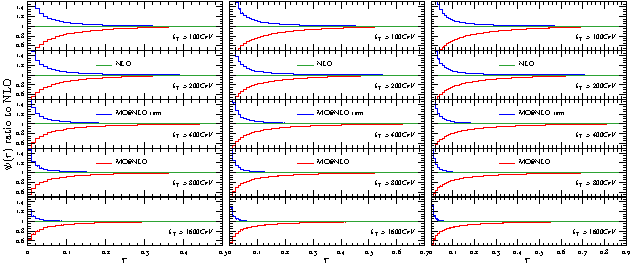
\includegraphics[width=\textwidth]{plots/shapes/hj/hjshapes-crop.pdf}\\
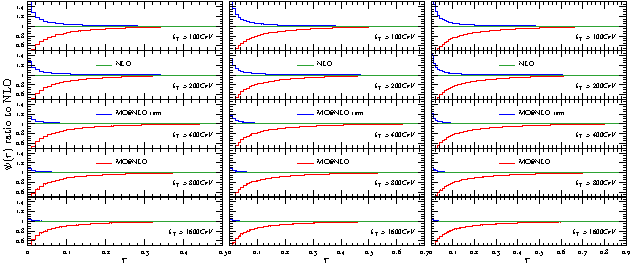
\includegraphics[width=\textwidth]{plots/shapes/zj/zjshapes-crop.pdf}\\
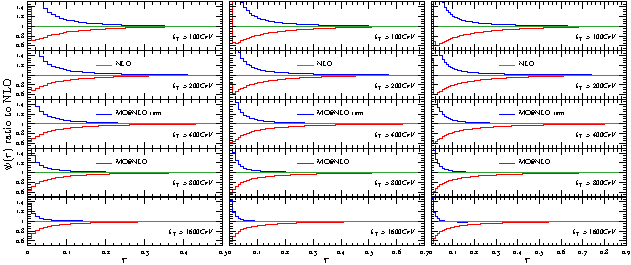
\includegraphics[width=\textwidth]{plots/shapes/jj/jjshapes-crop.pdf}
\caption{Jet shapes for Higgs and Z plus jets and inclusive jets}
\end{figure}

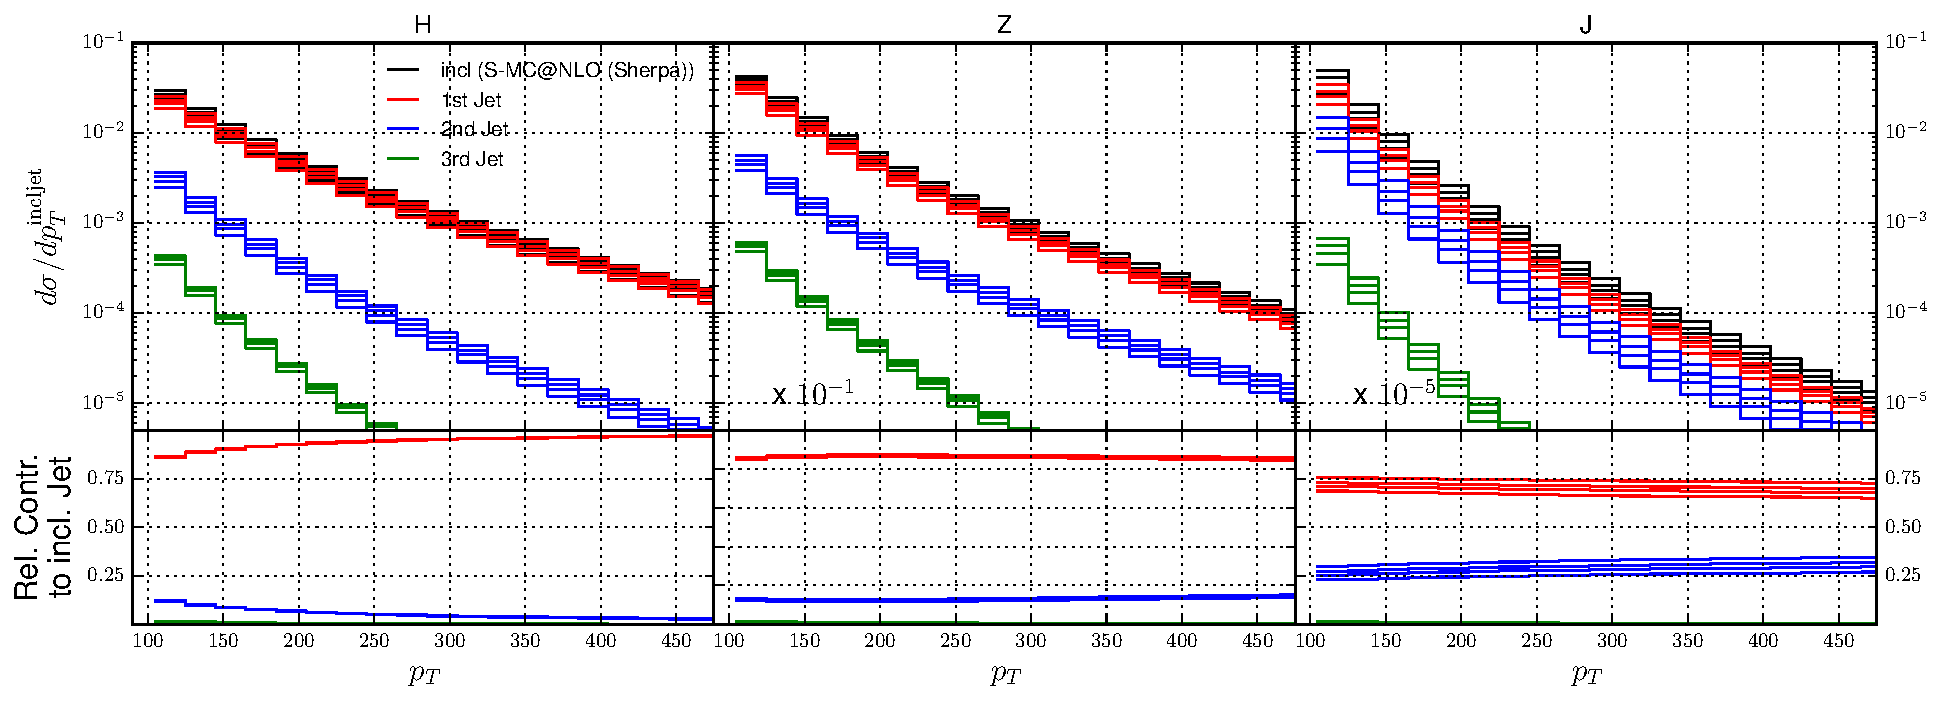
\includegraphics[width=\textwidth]{plots/Comparison_Contributions.pdf}
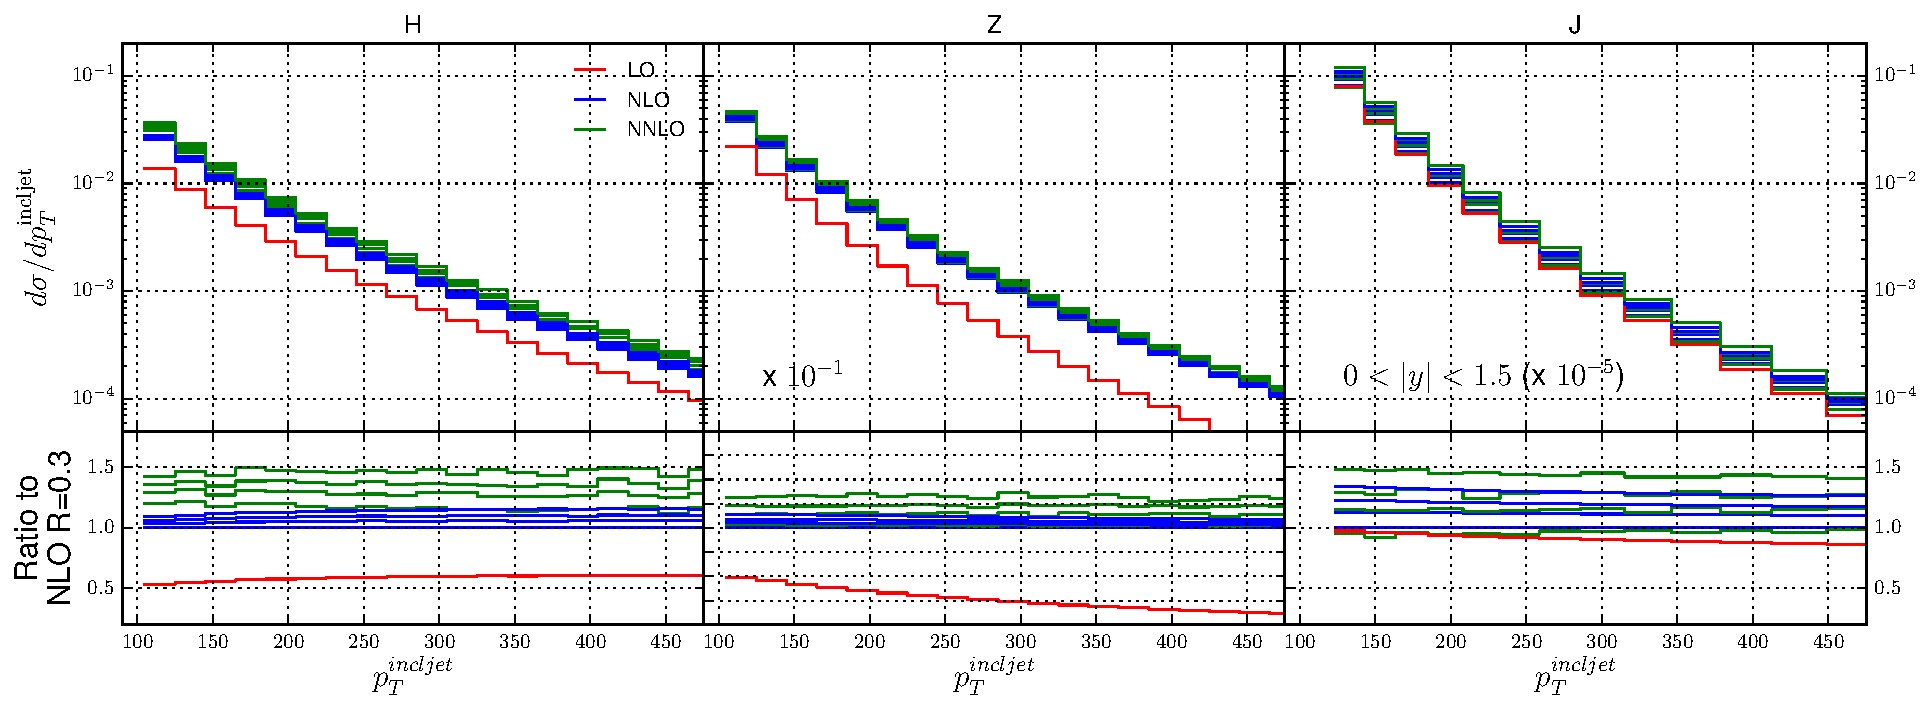
\includegraphics[width=\textwidth]{plots/Comparison_Plot.pdf}
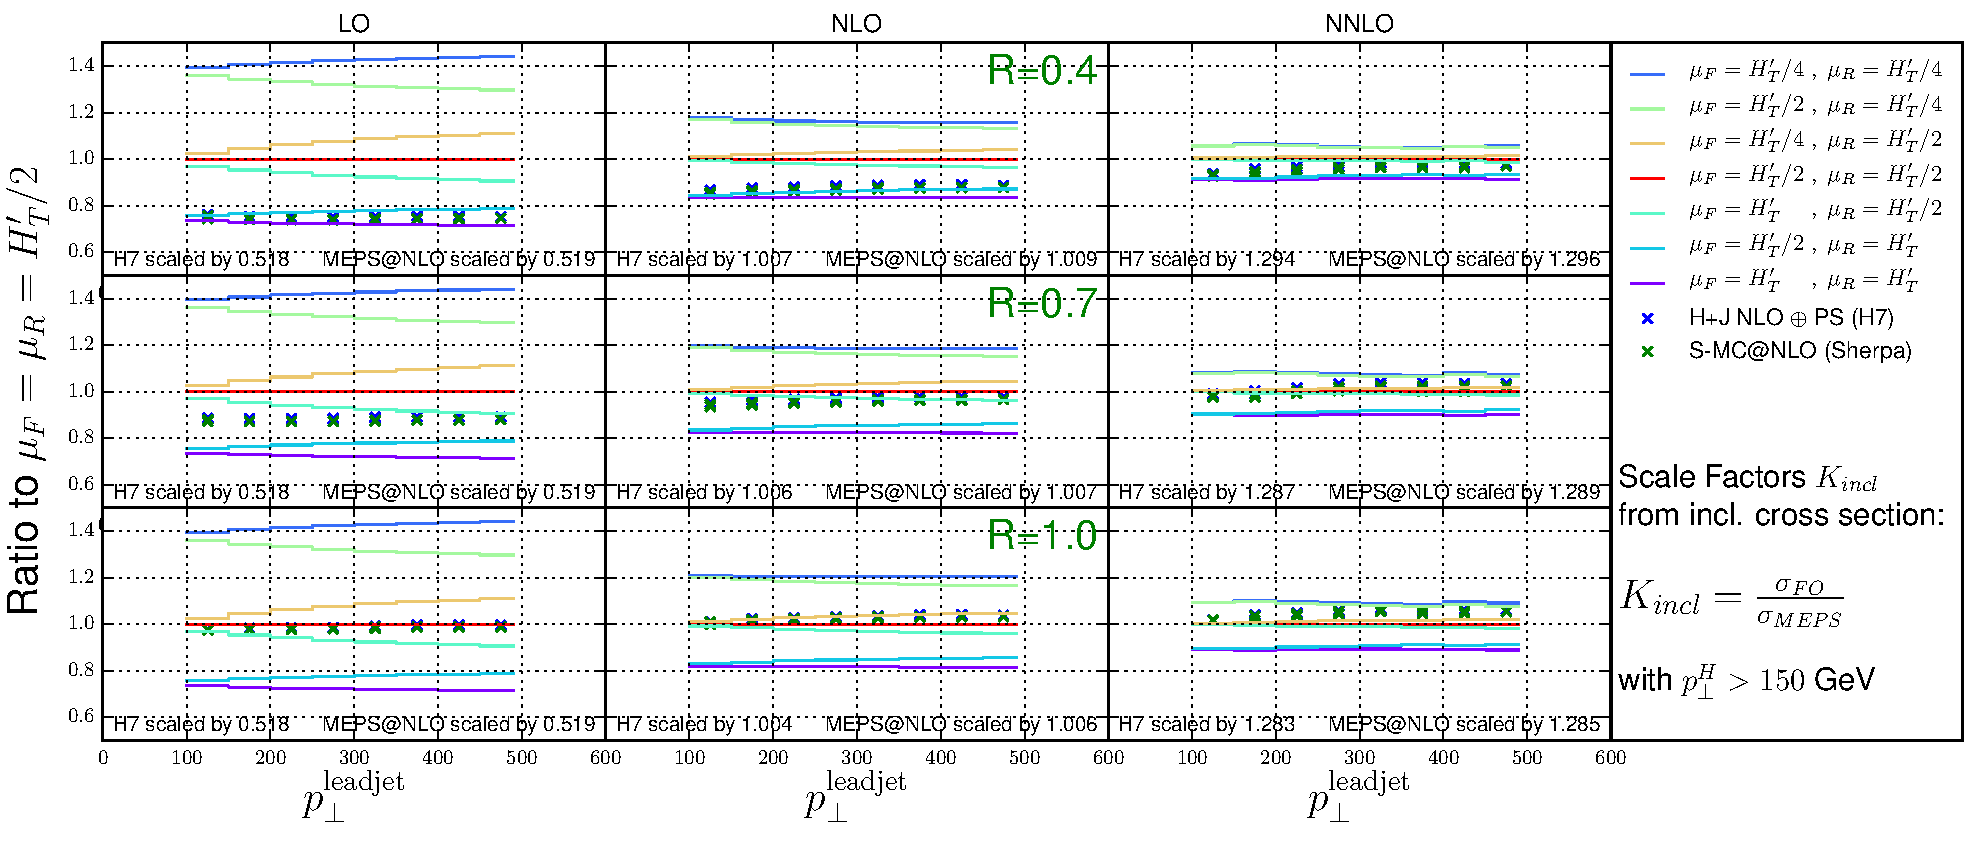
\includegraphics[width=\textwidth]{plots/Fig_V_16_Higgs.pdf}
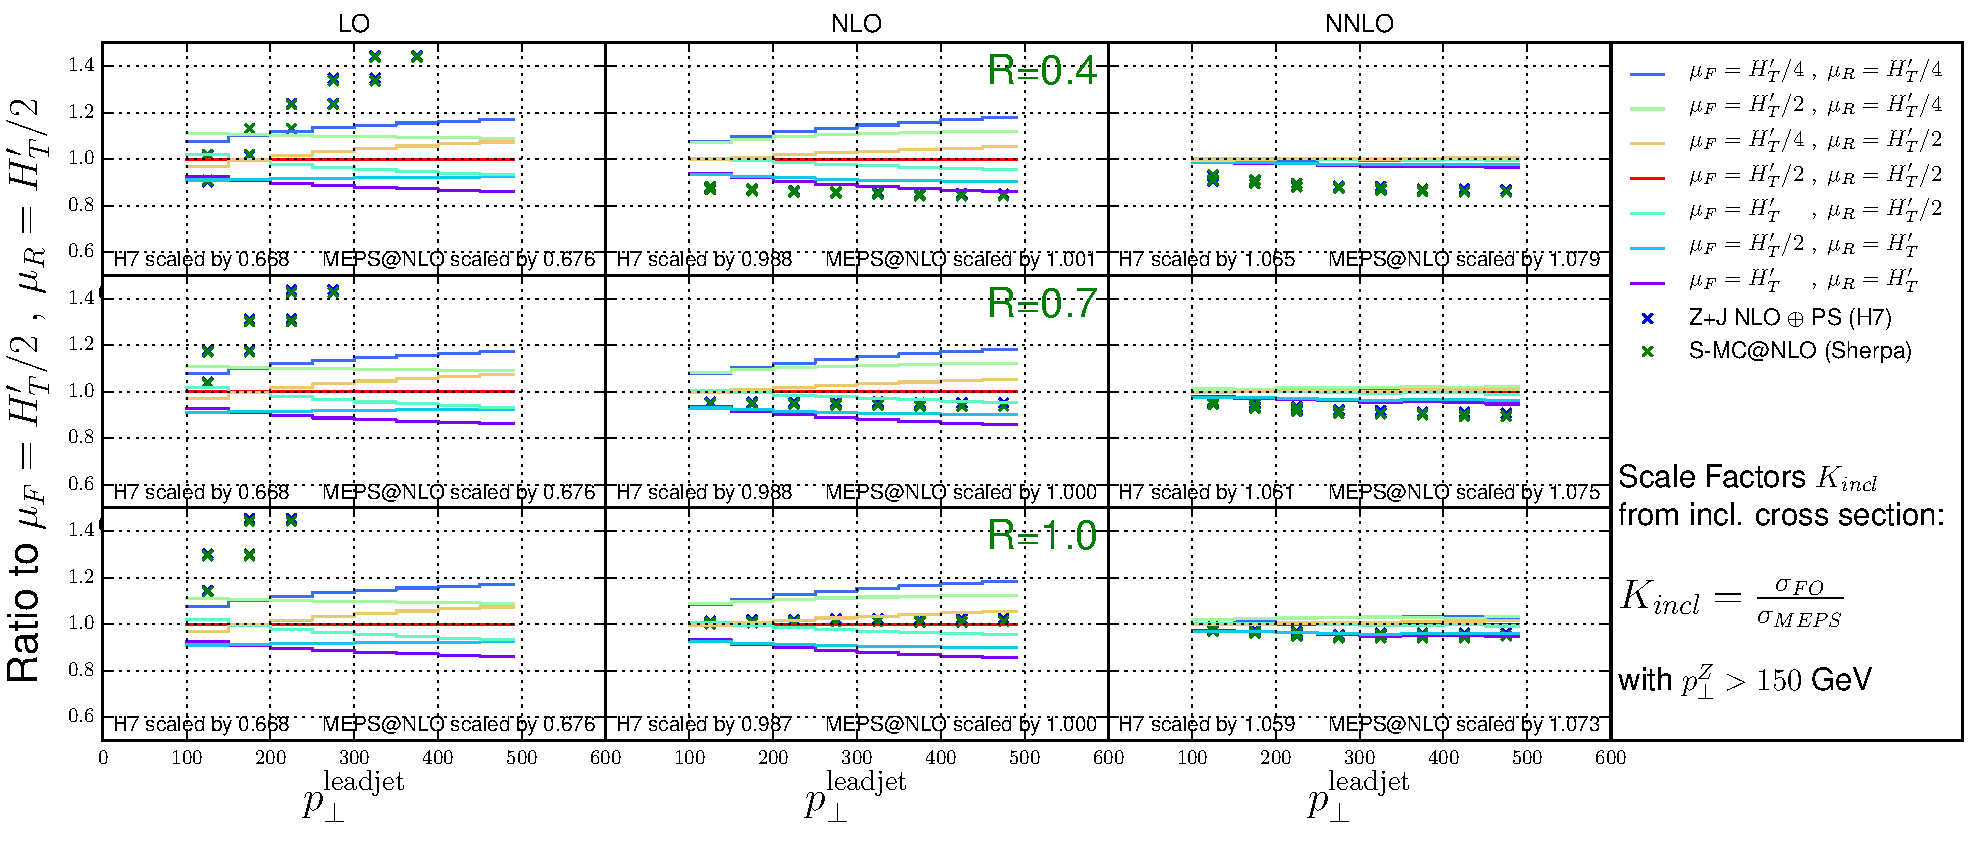
\includegraphics[width=\textwidth]{plots/Fig_V_16_ZJ.pdf}
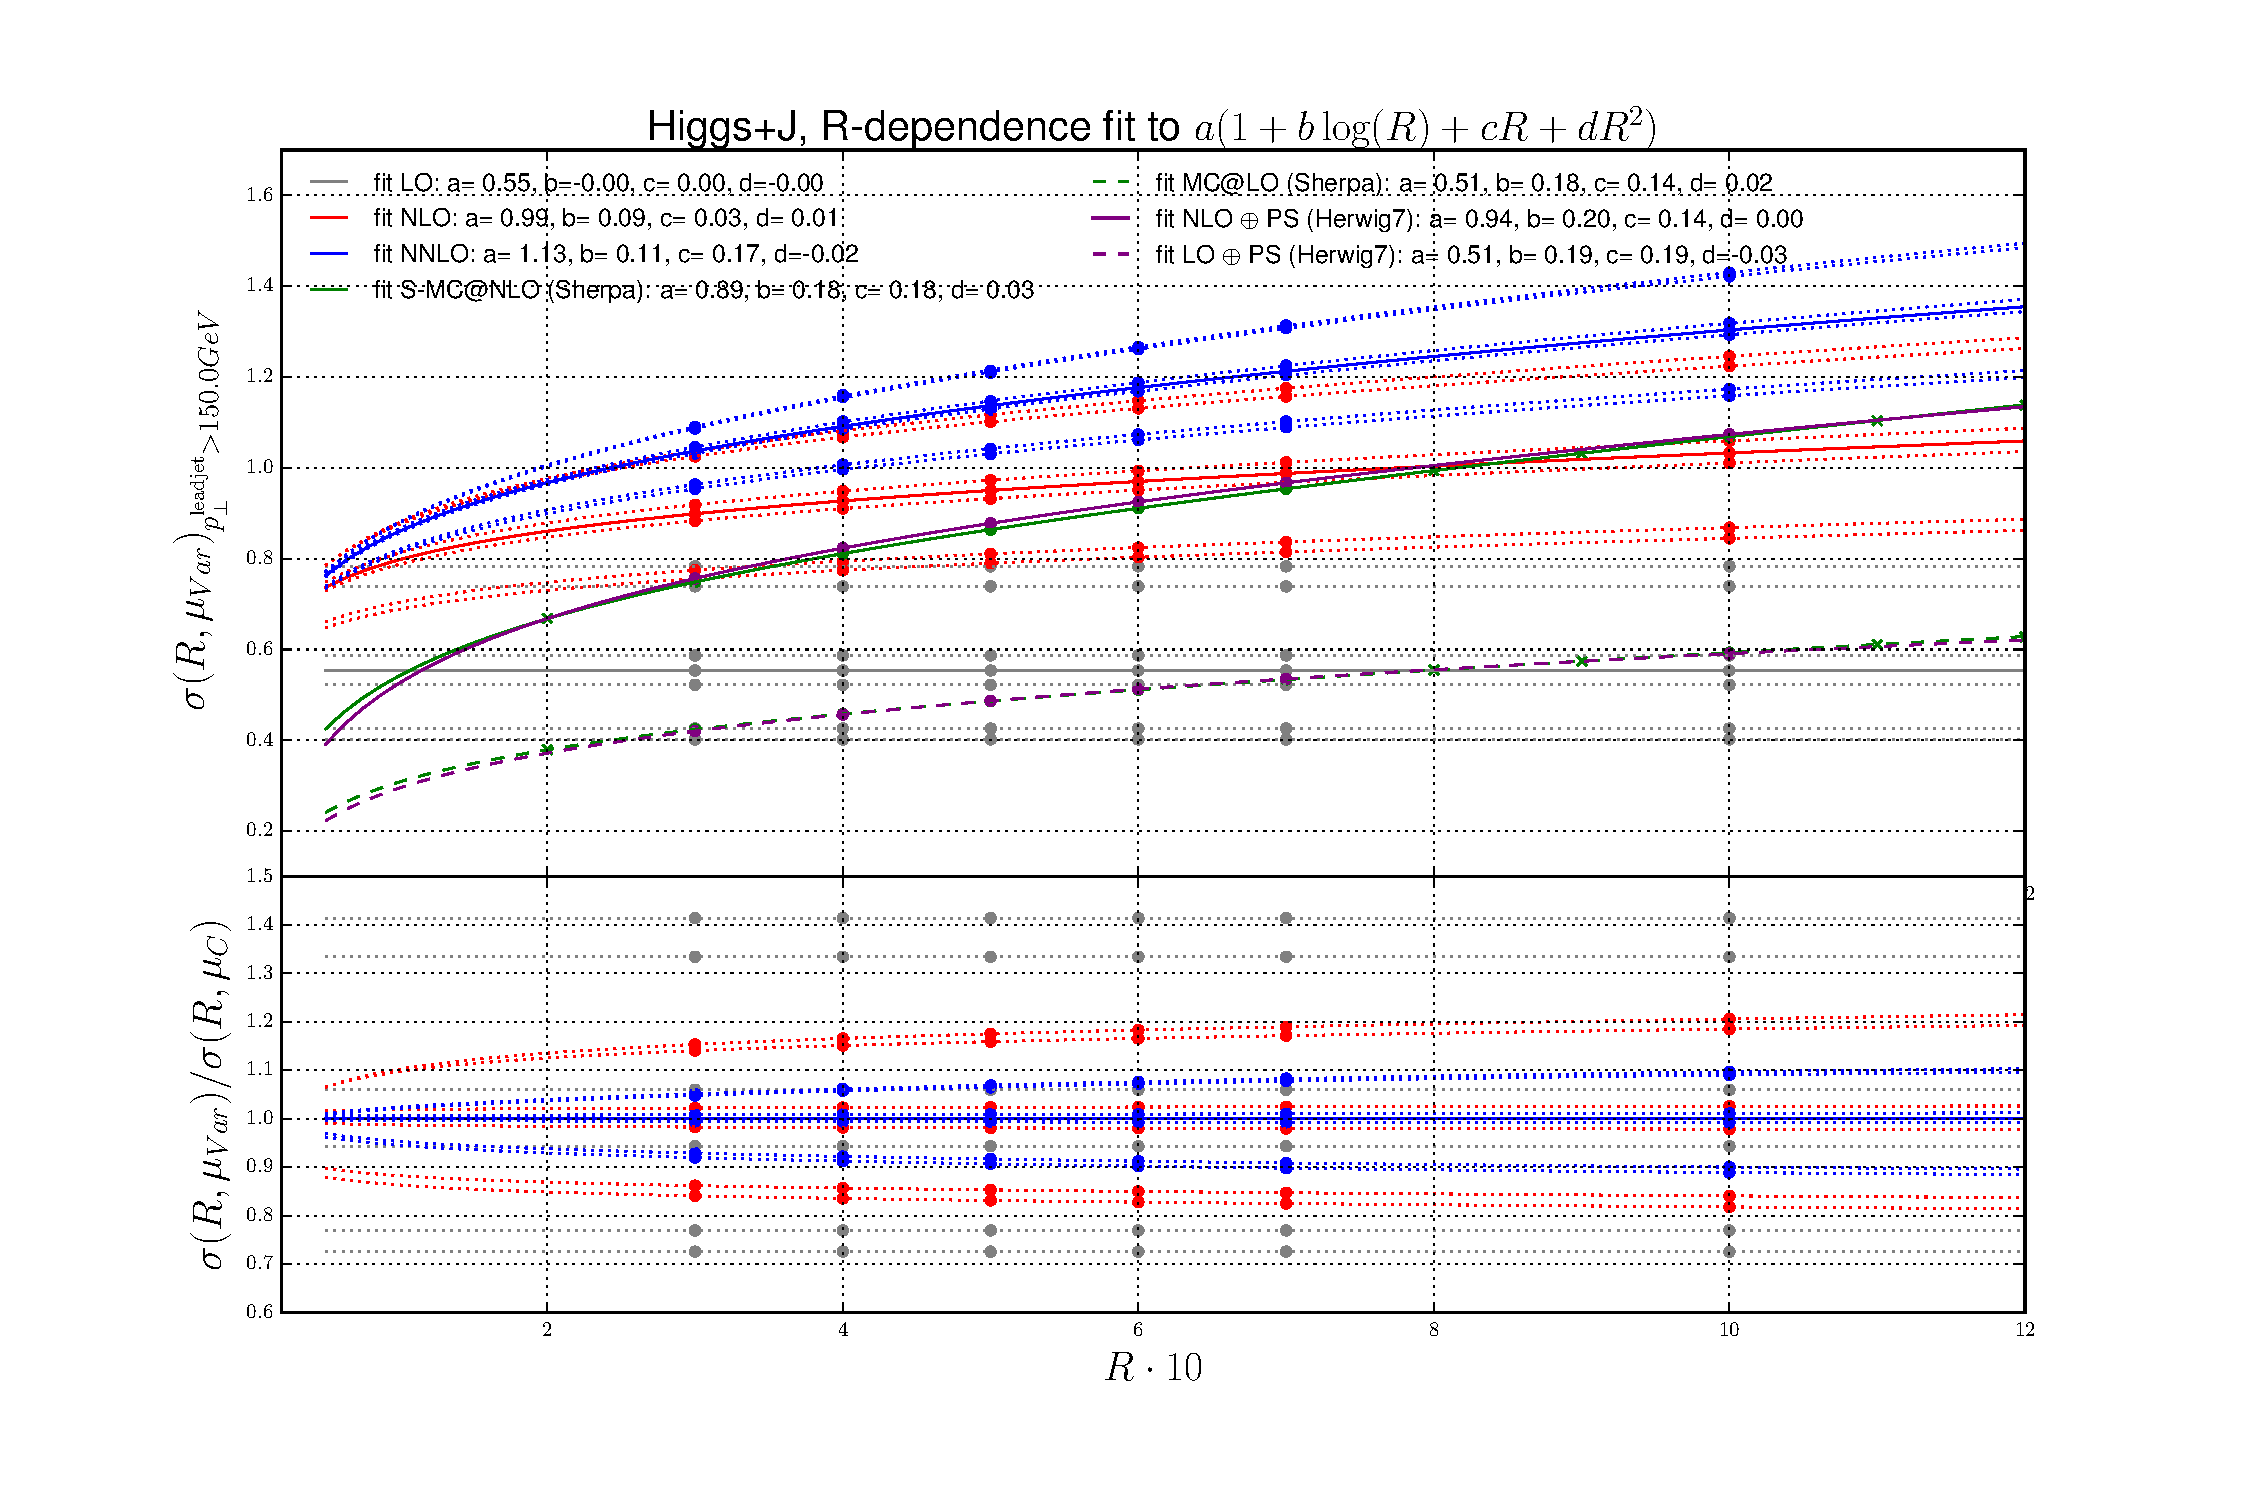
\includegraphics[width=\textwidth]{plots/Fig_V_17_Higgs.pdf}
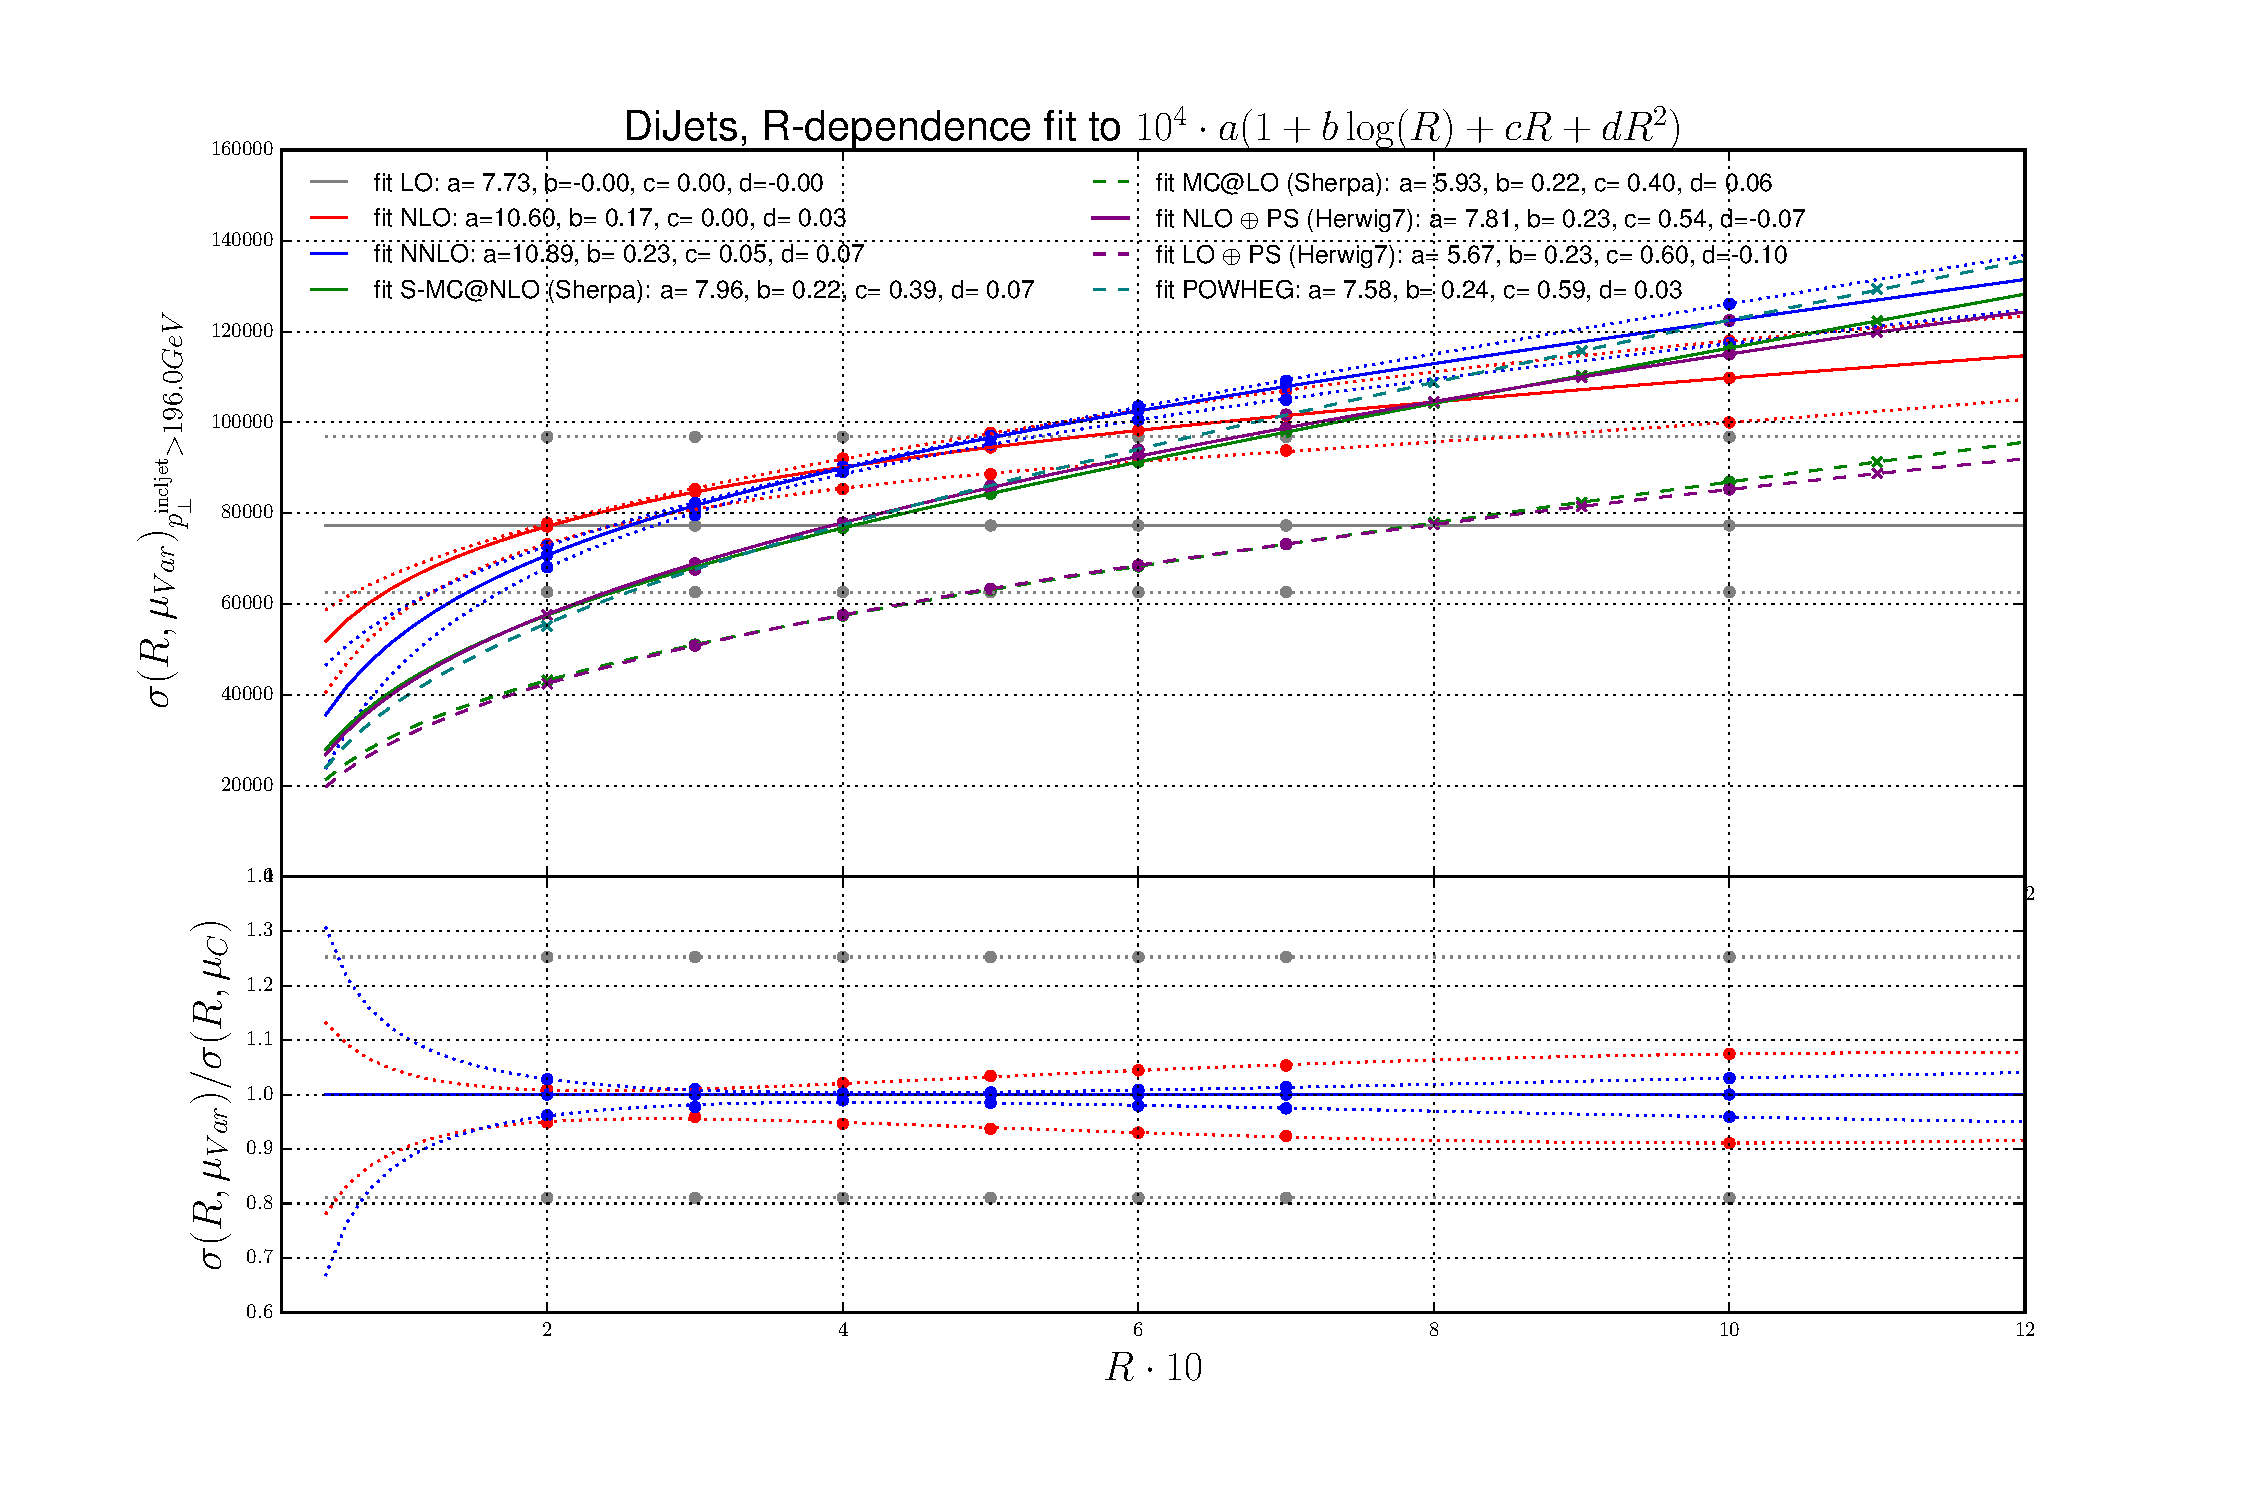
\includegraphics[width=\textwidth]{{plots/Fig_V_17_InclJet_196.0}.pdf}
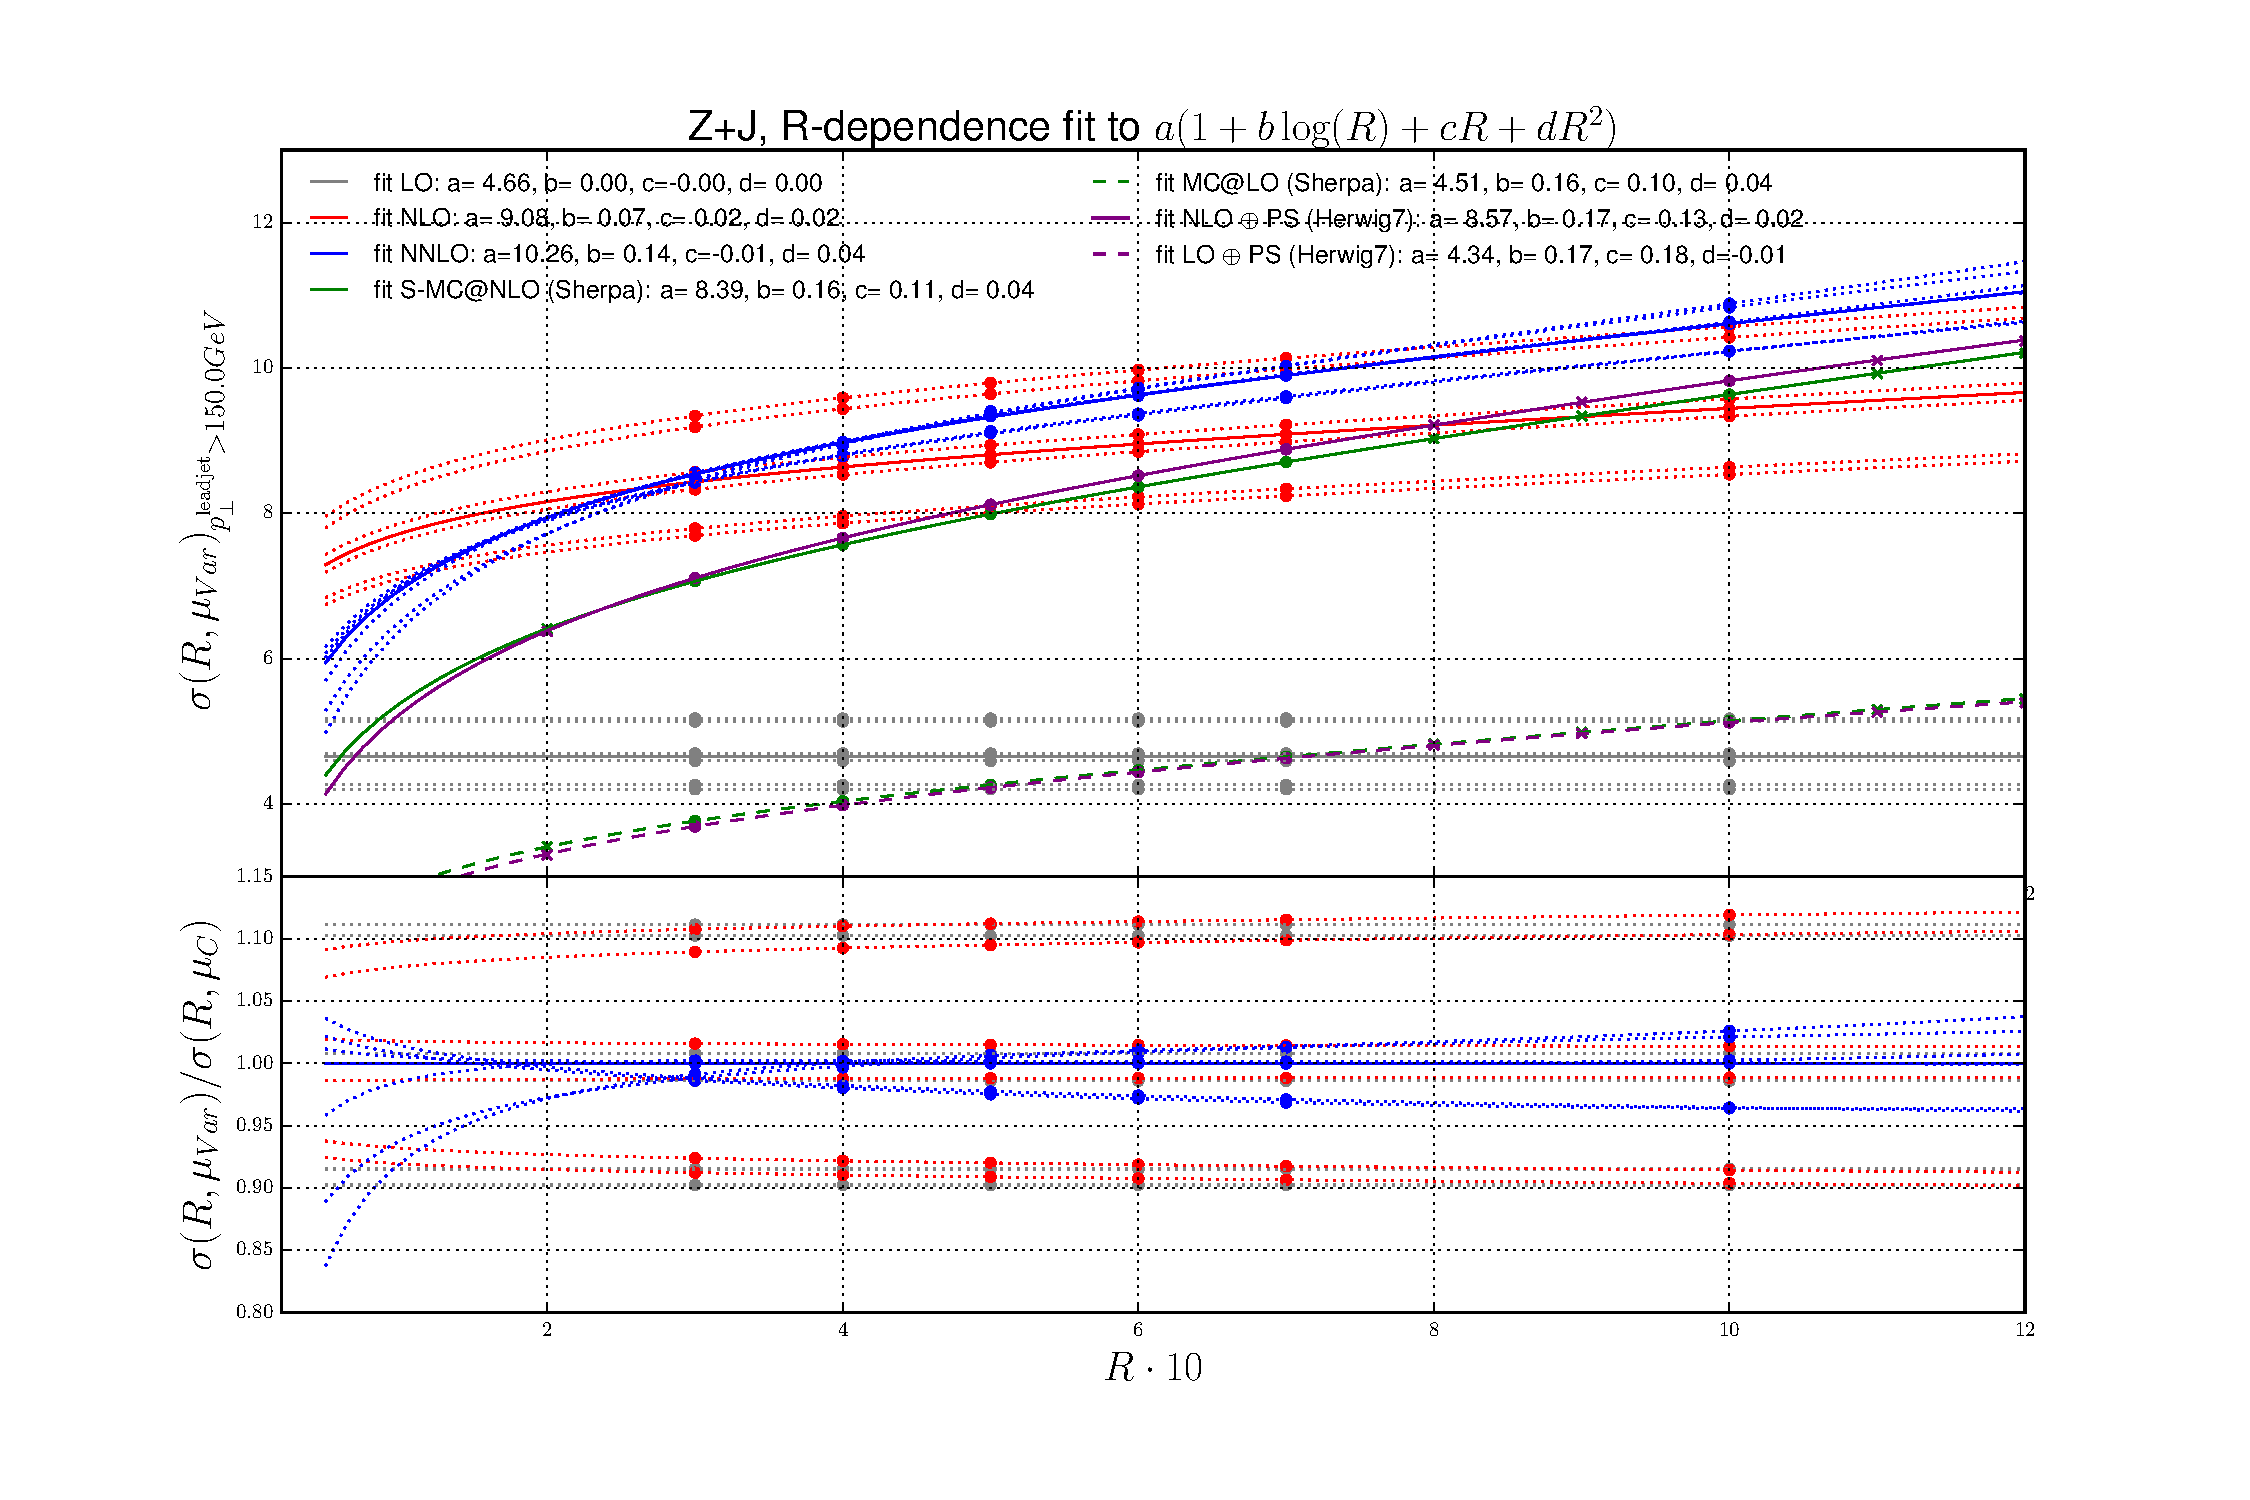
\includegraphics[width=\textwidth]{plots/Fig_V_17_Z.pdf}
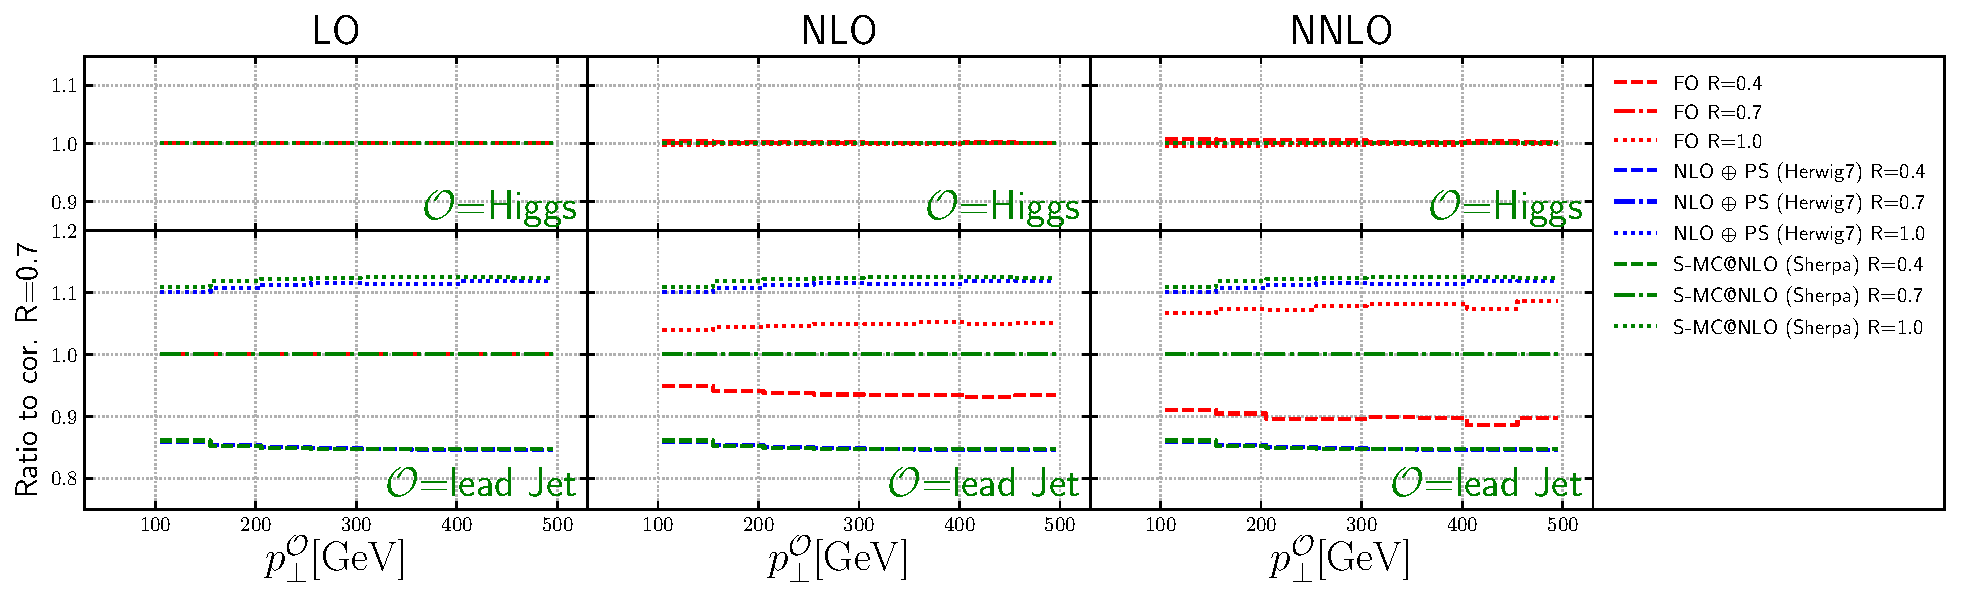
\includegraphics[width=\textwidth]{plots/Fig_V_18_Higgs.pdf}
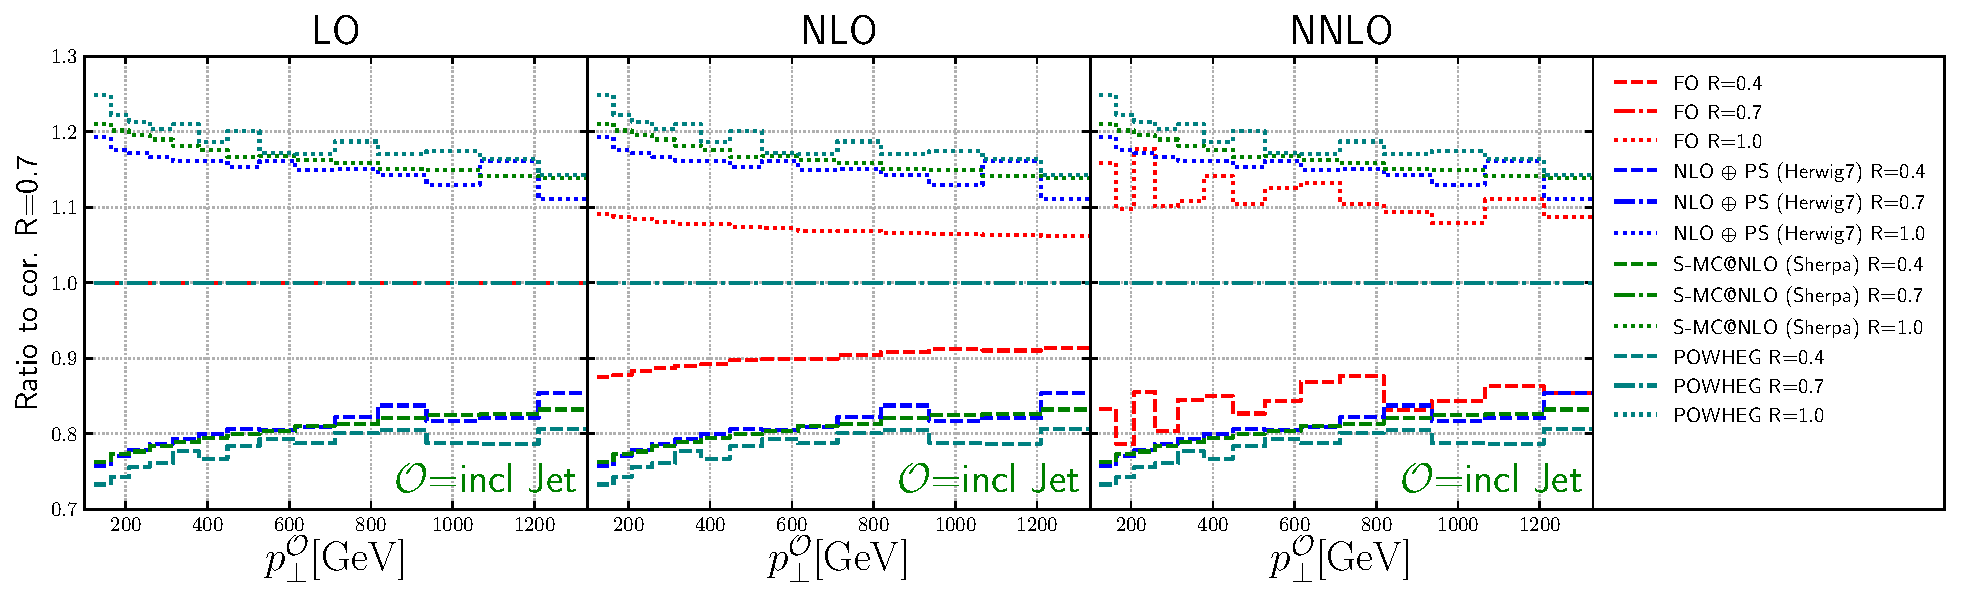
\includegraphics[width=\textwidth]{plots/Fig_V_18_inclJet.pdf}
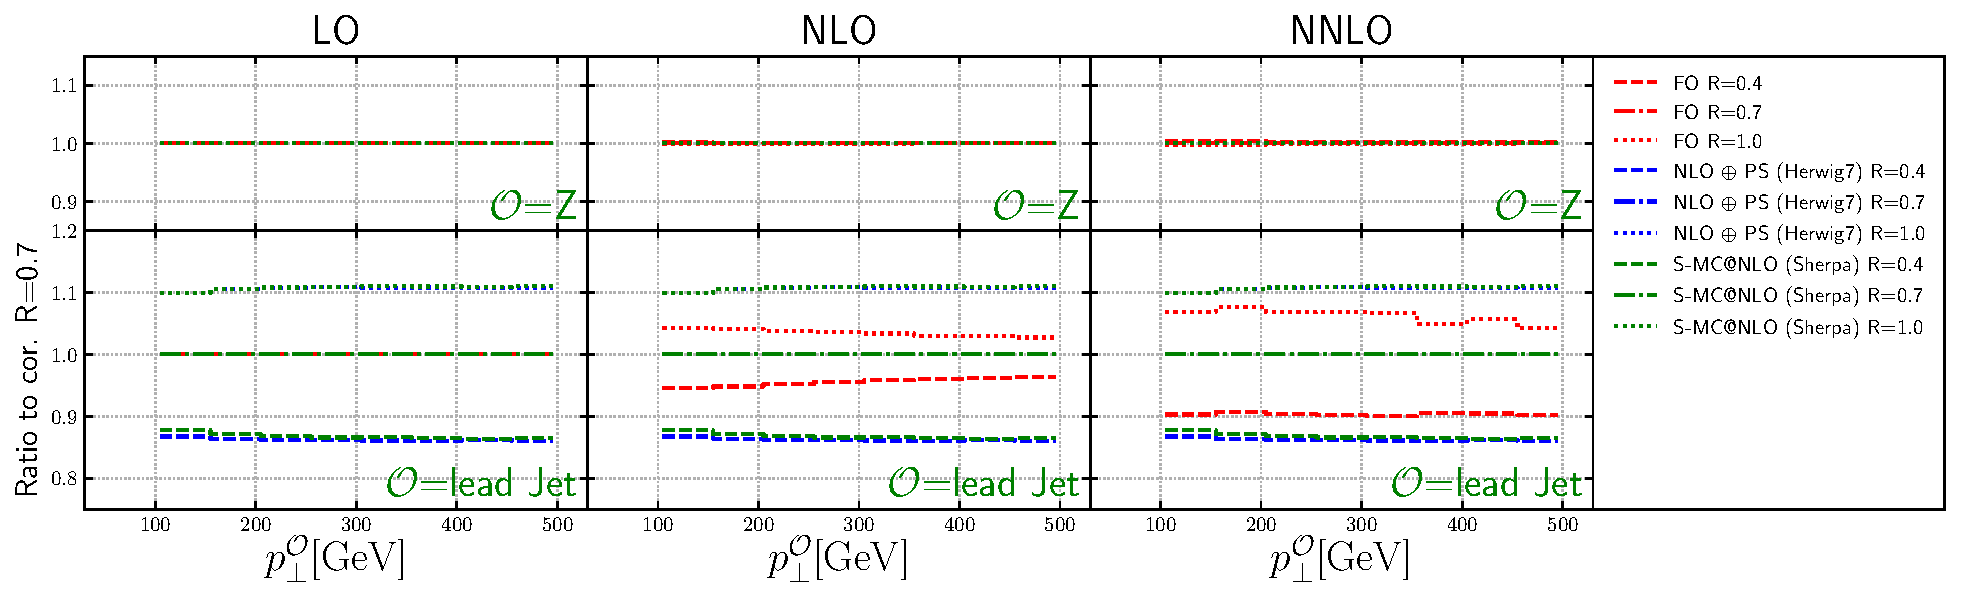
\includegraphics[width=\textwidth]{plots/Fig_V_18_Z.pdf}

\bibliography{journal.bib}

\end{document}
